\documentclass[thesis.tex]{subfiles}

\begin{document}

\chapter{Evaluation}\label{chap:eva}
This chapter will evaluate the proposed algorithms both from a performance and a quality perspective.
In the last section we try to compare our technique to others.
However, as we were not able to implement comparable implementations within the bounds of this project, we can only provide comparisons on an abstract level.

\section{Test Setup \& Scenes} \label{sec:eva:setup}
All tests were rendered using a Nvidia GTX670 desktop graphics card.
The test machine contains a Intel i7-3770 CPU and uses Windows 8 64bit as OS.

\begin{figure}
\centering
\begin{subfigure}[b]{0.8\textwidth}
\centering
\includegraphics[width=\textwidth]{eva/scenes/sponza}
\caption{\dataset{Sponza}}
\end{subfigure}
\\
\begin{subfigure}[b]{0.8\textwidth}
\centering
\includegraphics[width=\textwidth]{eva/scenes/sibenik}
\caption{\dataset{Sibenik}}
\end{subfigure}
\\
\begin{subfigure}[b]{0.8\textwidth}
\centering
\includegraphics[width=\textwidth]{eva/scenes/republique}
\caption{\dataset{Republique}}
\end{subfigure}
\caption{Overview over our three main test scenes.}
\label{fig:testscenes}
\end{figure}
\autoref{fig:testscenes} gives an overview over the main test scenes used in this chapter (and throughout the thesis).
We use McGuire's \cite{bib:McGuire2011Data} version of the well known Crytek \dataset{Sponza} scene which was modeled by Frank Meinl.
For a better fit into our physically based pipeline we used the freely provided texture set  by Alexandre Pestana \cite{bib:sponzapbr}.
Additionally, we placed a continuously rotating Utah teapot with a custom metal-like texture in the scene to show-case specular reflections on a curved surface with varying metallic and roughness values.
\\
The \dataset{Sibenik} cathedral scene is as well from McGuire's database \cite{bib:McGuire2011Data}.
To fill the empty space, we added a dinosaur skeleton from the "Natural History Museeum" modelled by Alvara Luna Bautista and Joel Anderson (available at \url{http://www.3drender.com/challenges/}).
\\
The \dataset{Republique} scene was extracted from a unity tech demo for the game "République Remastered" by Camouflaj.
The entire demo is freely available on the unity assetstore \cite{bib:republique}.

\section{Parameter Overview}
How our approach performs depends on several parameters.
To make this chapter more readable and make comparisons easier, we use a standard configuration on all parameters that are not mentioned explicitly.
Those defaults are annotated in brackets in this list:
\begin{easylist}
\ListProperties(Hide=100, Hang=true, Progressive=4ex, Space=0.0ex, Space3=-0.5ex, Space*=-0.5ex, Style*=$\bullet\,$,
Style2*=\textbf{--} ,Style3*=$\circ$ ,Style4*=\tiny$\blacksquare$ )
# general
## screen resolution ($1920\times1080$)
## number of lights (a single spot light)
## reflective shadow map resolution (rendering $1024^2$, indirect light $64^2$)
## number of SH bands for diffuse lighting (2 bands)
## number of active caches
### cache address volume resolution ($32^3$)
### cascading settings (4 cascades, last cascade covers always entire scene)
### camera
# shadowing
## shadow lod (2)
## voxel resolution ($128^3$)
# specular
## specular environment map resolution ($16^2$)
## direct write or cached write (direct write)
\end{easylist}
This chapter tries to give insights on their effects.
We limit our observation to meaningful ranges and do not experiment with arbitrary combinations.

 \todo{write why voxel res is bad}

\section{Performance}
In this section the performance and scalability of our approach is examined.
We measure primarily frame times in milliseconds.
To be able to evaluate how specific parts of our algorithm perform, we use multi-buffered OpenGLs timer query functionality to check how long a series of calls take to finish on the GPU (\texttt{GL\_TIME\_ELAPSED}) without stalling it.
The sum of timings from multiple commands may exceed the time a frame takes, since the GPU might work on multiple commands at a time.
However, in our tests this overlap seems to play a minor role since most tasks are either very computational intense or are depending on each other which prohibits parallel command execution.
\\
In general such measurements can slow down the rendering process.
For our scenarios though, we did not measure any drops the independently measured framerate with activated timer queries.

\subsection{General Breakdown}
First we want to provide a general overview over how long the different steps of our rendering pipeline usually take.
For this, we measure all timings along 30 seconds camera flights through our test scenes using the default settings mentioned in \autoref{sec:eva:setup}.
The first set of graphs in \autoref{fig:frameratebreakdown:specoff} shows timings without and the second in \autoref{fig:frameratebreakdown:specoff} with indirect specular reflections.
The stacked area plots in the graph are sorted in the order in which the respective passes are issued, starting with the GBuffer creation (light green) at the bottom and ending with the cache interpolation on top (beige).
The black line at the top of all plots shows the total duration for each recorded frame.
Note that there is a small white gap bellow this line which represents the duration of all overheads that were not measured explicitly like tonemapping, several uniform buffer updates and backbuffer output.

As easily can be seen, the indirect specular lighting increases the costs of the indirect lighting pass (dark yellow) considerably while the additional mipmapping of the specular environment map is very cheap.
Since the light does not move in these tests, the rendering of the (reflective) shadow map (dark grey) is constant over time.
The duration both the voxelization pass and its blending + mipmapping is constant as well since there are no changes over time in resolution, number of written cells or geometrical complexity of the scene.
More surprisingly, there are also almost no changes over time in the cache allocation pass (bright yellow) even when the cache lighting pass (dark yellow) is significantly slower which hints a higher number of light caches.
Since the main influence to this and the other two cache related passes is the number of of active caches we will investigate this further in the next section on cache count. 
The strong changes in the duration of the gbuffer creation pass (especially in \dataset{Sponza}) stem from varying overdraw along the camera path. \todo{insert reference to videos of the paths}

\begin{figure}
\centering
\includegraphics[width=\textwidth]{eva/breakdown/specoff.pdf}
\caption{Breakdown of frame timings with a moving camera over time (30s) for indirect diffuse lighting with shadowing.}
\label{fig:frameratebreakdown:specoff}
\end{figure}
\begin{figure}
\centering
\includegraphics[width=\textwidth]{eva/breakdown/specon.pdf}
\caption{Breakdown of frame timings with a moving camera over time (30s) for indirect diffuse \& \emph{specular} lighting with shadowing.}
\label{fig:frameratebreakdown:specon}
\end{figure}

\subsection{Cache Count}
Retrieving the current cache count from the GPU is a very costly operation unless extensive multi-buffering is used to avoid stalls (keeping the count in a different buffer every frame to ensure to perform reads only on an unused one).
Therefore, we measured the cache count over time separately and combined the results in the graphs seen in \autoref{fig:cachecountovertime}.

\begin{figure}
\centering
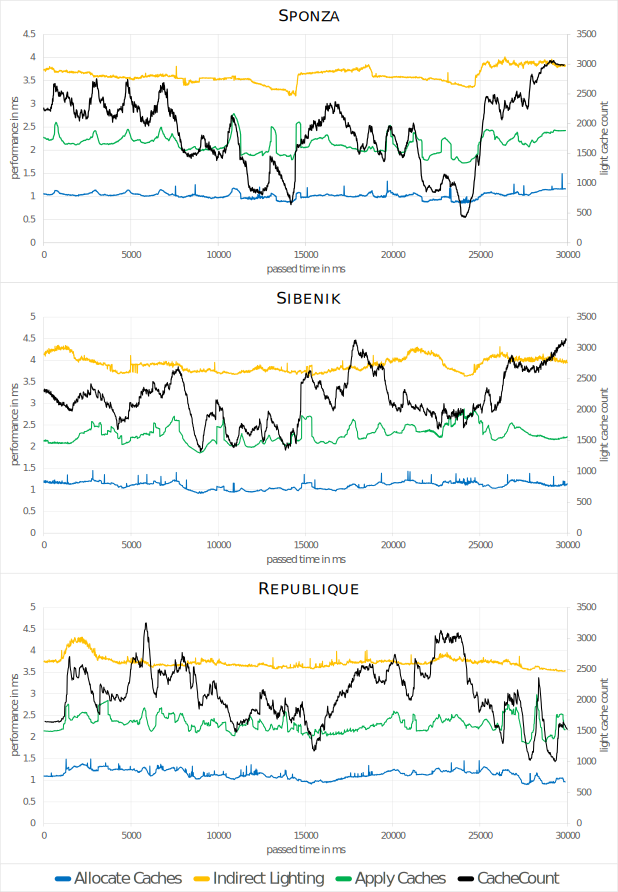
\includegraphics[width=\textwidth]{eva/cachecountovertime/combined.pdf}
\caption{Visualization of the influence of cache count (black) to all relevant passes over time (30s), using the same camera flights and settings as in \autoref{fig:frameratebreakdown:specoff}.}
\label{fig:cachecountovertime}
\end{figure}

Surprisingly, there seems to be only slight correlation between the duration of the cache lighting pass and the number of caches.
The duration of the allocate pass is rather stable over time and only the apply cache pass shows a slight and very unsteady correlation to the cache count.
\\
The steadiness of the cache allocation pass comes most likely from the fact that on average every thread group performs a single cache allocation attempt regardless of the cache count (since it does not go high enough in our scenarios).
Weather an attempt is redundant or not might not as important for the runtime.
The cache apply pass on the other hand has a strict control flow, i.e. it executes the same code insensitive to the number of caches.
This leaves only the changing number of cache misses as reasonable explanation for its behavior.
Clearly, the main bottleneck of the cache lighting pass in the preceding tests is not the raw number (within the tested bounds) of caches to be lit, but another factor that changed along the tested camera paths.
To reduce the number of influences we ran the same experiment in the \dataset{Sponza} scene again with disabled indirect shadow.

\begin{figure}
\centering
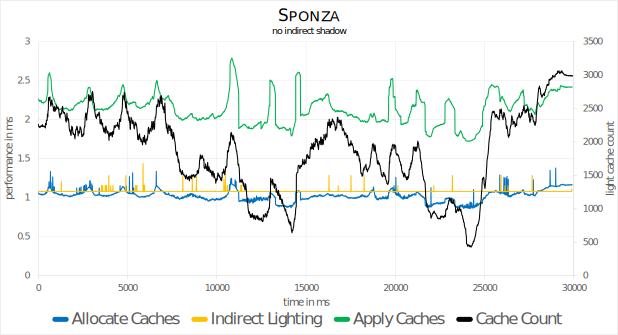
\includegraphics[width=\textwidth]{eva/cachecountovertime/sponza_noshadow.pdf}
\caption{Cache count (black) in comparison to indirect lighting passes with inactive indirect shadowing (camera path and other settings as in \autoref{fig:frameratebreakdown:specoff}).}
\label{fig:cachecountovertime:noshadow}
\end{figure}

The results, seen in \autoref{fig:cachecountovertime:noshadow}, show a even more extreme picture:
Now the duration of the caching pass is almost completely constant, while correlations of the cache count and the performance of the other two parts are much better visible.
Naturally we suspected a bug in the implementation of the light caching pass that is expected to a have linear performance characteristic in respect to the number of active light caches.
However, more experiments with higher cache counts show that there is in fact such a linear correlation.
This time we chose a fixed view point in the \dataset{Sponza} scene, using the default non-specular settings and measured the performance (and cache count) for different CAV resolutions.
\todo{graph showing our experiment}
Our implementation uses 512 threads per group during the cache lighting pass.
This is the lowest theoretical granularity to which the performance of this pass can react, since the shared memory optimization (see \autoref{label} \todo{}) enforces that all threads of a group remain active.
Obviously though, due to some characteristics of our graphics card (or driver), the measured granularity is much coarser, especially for a low number of thread groups.
More experiments with different thread group sizes would be necessary for a deeper insight into this matter.

The experiment also % confirms our hypothesis on the behaviour of the allocate cache pass, .....................



\todo{Experiments considering cascading? Impact of transitions?}

\subsection{Resolution Dependence}
Examine effect of resolution on prepare and apply passes.

\subsection{Indirect Shadow}


\subsection{Indirect Specular}

\newpage

\section{Quality}
% phenomelogical: "Quality of light, shadow, etc." - which parameters need to be tweaked

\subsection{Sources of Error and Groundtruth Comparision}
Shadow heuristic check! (try to use only one)

\subsection{Artifacts}
regular placement of caches, jaggies,
shadow jaggies,
/interpolation issues

shadow flickering?

\subsection{Temporal Coherency}


\section{Memory Consumption}

\section{Comparison to other Techniques} \label{sec:eva:comparisiontoother}

comparison table, similar to the one in radiance hints?

\subsection{Comparison to LightSkin}

\subfilebib % Makes bibliography available when compiling as subfile
\end{document}